% Enable warnings about problematic code
\RequirePackage[l2tabu, orthodox]{nag}

\documentclass{WeSTassignment}

% The lecture title, e.g. "Web Information Retrieval".
\lecture{Introduction to Web Science}
% The names of the lecturer and the instructor(s)
\author{%
  Prof.~Dr.~George~Martin\\{\normalsize\mailto{gmartin@uni-koblenz.de}} \and
  Jon~Snow\\{\normalsize\mailto{jsnow@uni-koblenz.de}}
}
% Assignment number.
\assignmentnumber{X}
% Institute of lecture.
\institute{%
  Institute of Web Science and Technologies\\%
  Department of Computer Science\\%
  University of Koblenz-Landau%
}
% Date until students should submit their solutions.
\datesubmission{November 17, 2017, 11:00 a.m.}
% Date on which the assignments will be discussed in the tutorial.
\datetutorial{November 24, 2017, 12:00 p.m.}

% Specify bib file location.
\addbibresource{bibliography.bib}

% For left aligned centerd boxes
% see http://tex.stackexchange.com/a/25591/75225
% ==============================================================================
% Document

\begin{document}

\maketitle
This assignment focuses on the topics of 1) \textbf{Hello World}, 2) \textbf{Plotting}.

For all the assignment questions that require you to write code, make sure to include the code in the answer sheet, along with a separate Python file. If you generate a plot from your Python script, please add them in the answer sheet.\\ \\ 

%Please mention your team Names here: 
Team Name: XXXX


\section{Hello World \hfill (10 points)}
Your task is to print ``Hello, World!'' on the screen.

\subsection*{Solution}
%solution-start
\subsubsection*{hello\_world.py}
\lstinputlisting[language=Python, breaklines=true]{hello_world.py}
%solution-end
%-------------------------------------------------------------------------------

\section{Plotting \hfill (15 points)}
Plot the function $y=x^2$ in the domain $[-2,2]$.
You are allowed to use the packages \texttt{numpy} and \texttt{matplotlib}.

\subsection*{Solution}
%solution-start
\subsubsection*{plot.py}
\lstinputlisting[language=Python, breaklines=true]{plot.py}
\subsubsection*{plot.png}
\begin{center}
  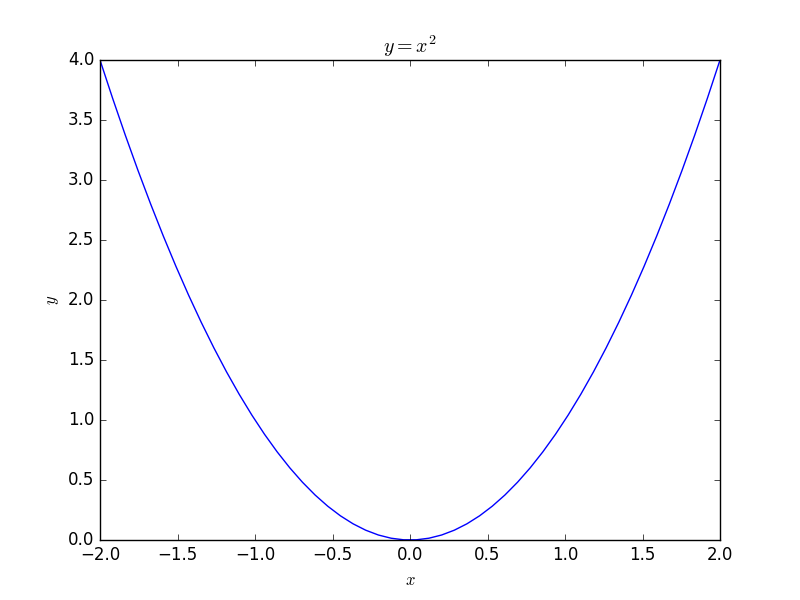
\includegraphics[width=0.75\textwidth]{plot.png}
\end{center}
%solution-end
%-------------------------------------------------------------------------------

\makefooter

\end{document}

